\section{Реализация}

\subsection{Архитектура приложения}

Приложение построено на основе архитектурного паттерна \\ 
\textbf{Model/View/Controller (MVC)}, который обеспечивает разделение ответственности между компонентами системы:

\begin{itemize}
    \item \textbf{Model (Модель)} — классы \texttt{Contact}, \texttt{ContactManager}, \texttt{ContactTableModel}, отвечающие за хранение и управление данными;
    \item \textbf{View (Представление)} — класс \texttt{MainWindow} и используемые виджеты Qt (\texttt{QTableView}, \texttt{QLineEdit}, \texttt{QPushButton} и др.), отвечающие за отображение данных пользователю;
    \item \textbf{Controller (Контроллер)} — методы-слоты класса \texttt{MainWindow}, обрабатывающие пользовательский ввод и взаимодействие с моделью.
\end{itemize}

Дополнительно используется класс \texttt{Validator} для валидации данных и \texttt{QSortFilterProxyModel} для фильтрации и сортировки данных в таблице. \\

Структура директорий проекта:

\begin{lstlisting}[style=cppstyle, caption={Структура директорий.}]
lab8/
├── CMakeLists.txt
├── main.cc
├── core/
│   ├── include/
│   │   ├── Contact.h
│   │   ├── ContactManager.h
│   │   ├── ContactTableModel.h
│   │   └── Validator.h
│   └── src/
│       ├── ContactManager.cc
│       ├── ContactTableModel.cc
│       └── Validator.cc
├── ui/
│   ├── include/
│   │   └── MainWindow.h
│   └── src/
│       ├── MainWindow.cc
│       ├── MainWindowUI.cc
│       └── MainWindowLogic.cc
└── data/
    └── contacts.json
\end{lstlisting} 

\newpage

Структурная схема взаимодействия компонентов представлена на рис. 1.

\begin{figure}[H]
    \centering
    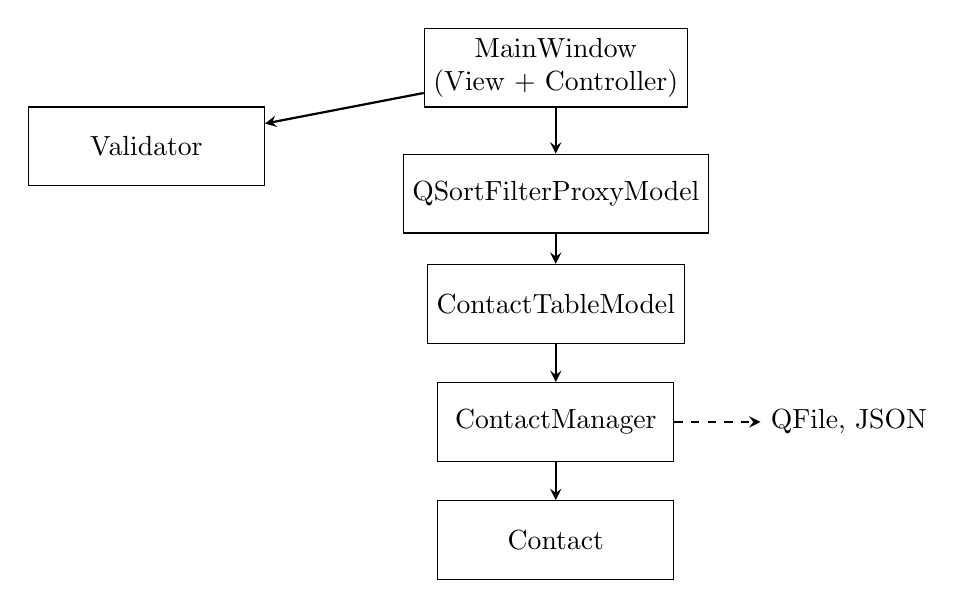
\begin{tikzpicture}[
        box/.style={rectangle, draw, minimum width=3cm, minimum height=1cm, align=center},
        arrow/.style={->, >=stealth, thick}
    ]
        \node[box] (ui) at (1.2,4) {MainWindow\\(View + Controller)};
        \node[box] (proxy) at (1.2,2.4) {QSortFilterProxyModel};
        \node[box] (model) at (1.2,1) {ContactTableModel};
        \node[box] (manager) at (1.2,-0.5) {ContactManager};
        \node[box] (contact) at (1.2,-2) {Contact};
        \node[box] (validator) at (-4,3) {Validator};
        
        \draw[arrow] (ui) -- (proxy);
        \draw[arrow] (proxy) -- (model);
        \draw[arrow] (model) -- (manager);
        \draw[arrow] (manager) -- (contact);
        \draw[arrow] (ui) -- (validator);
        \draw[arrow, dashed] (manager) -- ++(2.6,0) node[right] {QFile, JSON};
    \end{tikzpicture}
    \caption{Архитектура приложения}
    \label{fig:architecture}
\end{figure}


\subsection{Описание классов}

\subsubsection{Структура Contact}
\textbf{Contact} - структура, отвечающая за хранение одной записи контакта.

\begin{lstlisting}[style=cppstyle, caption={Contact}]

#pragma once 

#include <QString>
#include <QDate>
#include <QMap>
#include <QUuid>

//* служит моделью QTable
struct Contact {
    QString firstName_;
    QString lastName_;
    QString middleName_;
    QString adress_;
    QDate birthDate_;
    QString email_;
    QMap<QString, QString> phoneNumbers_;
};
\end{lstlisting}

\subsubsection{Класс ContactManager}

\texttt{ContactManager} — класс для управления коллекцией контактов. Инкапсулирует логику работы с данными и предоставляет интерфейс для работы с данными.

\begin{lstlisting}[style=cppstyle, caption={ContactManager}]
#pragma once 
#include <QList>
#include "Contact.h"

// * класс для управления коллекцией контактов
class ContactManager {
public:
    ContactManager() = default;
    ~ContactManager() = default;

    // * --- CRUD операции ---
    void addContact(const Contact& contact);                
    void removeContact(int index);                           
    void updateContact(int index, const Contact& contact);   

    // * --- геттеры, доступ к данным ---
    const QList<Contact>& getContacts() const;               
    QList<Contact>& getContactsMutable();                   
    int contactCount() const;                                
    Contact* getContact(int index);                        

    // * --- работа с данными ---
    bool loadFromFile(const QString& filePath);             
    bool saveToFile(const QString& filePath) const;    

private:
    QList<Contact> m_contacts; // основная коллекция для всех контактов 
};
\end{lstlisting}

\textbf{Псевдокод метода saveToFile:}

\begin{quote}
\textbf{Функция saveToFile(filePath):} \\
\hspace*{1em}создать пустой JSON-массив \texttt{contactArray} \\
\hspace*{1em}для каждого контакта в коллекции: \\
\hspace*{2em}создать JSON-объект \texttt{contactObject} \\
\hspace*{2em}записать все поля контакта в \texttt{contactObject} \\
\hspace*{2em}для каждого телефона в \texttt{phoneNumbers}: \\
\hspace*{3em}добавить пару (тип → номер) в \texttt{phonesObject} \\
\hspace*{2em}добавить \texttt{phonesObject} в \texttt{contactObject} \\
\hspace*{2em}добавить \texttt{contactObject} в \texttt{contactArray} \\
\hspace*{1em}создать JSON-документ из \texttt{contactArray} \\
\hspace*{1em}открыть файл по пути \texttt{filePath} для записи \\
\hspace*{1em}если файл успешно открыт: \\
\hspace*{2em}записать JSON-документ в файл \\
\hspace*{2em}закрыть файл \\
\hspace*{2em}вернуть \texttt{true} \\
\hspace*{1em}иначе вернуть \texttt{false}
\end{quote}

\textbf{Псевдокод метода loadFromFile:}

\begin{quote}
\textbf{Функция loadFromFile(filePath):} \\
\hspace*{1em}открыть файл по пути \texttt{filePath} для чтения \\
\hspace*{1em}если файл не открыт: \\
\hspace*{2em}вернуть \texttt{false} \\
\hspace*{1em}считать весь файл в переменную \texttt{data} \\
\hspace*{1em}закрыть файл \\
\hspace*{1em}разобрать \texttt{data} как JSON-документ \\
\hspace*{1em}если документ невалидный или не является массивом: \\
\hspace*{2em}вернуть \texttt{false} \\
\hspace*{1em}очистить текущую коллекцию контактов \\
\hspace*{1em}для каждого элемента в JSON-массиве: \\
\hspace*{2em}создать новый объект \texttt{Contact} \\
\hspace*{2em}считать все поля из JSON-объекта \\
\hspace*{2em}для каждого телефона в \texttt{phonesObject}: \\
\hspace*{3em}добавить пару (тип → номер) в \texttt{contact.phoneNumbers} \\
\hspace*{2em}добавить \texttt{contact} в коллекцию \\
\hspace*{1em}вернуть \texttt{true}
\end{quote}

\subsubsection{Класс ContactTableModel}

\texttt{ContactTableModel} — адаптер между \texttt{ContactManager} и \texttt{QTableView}. Наследуется от абстрактного класса \texttt{QAbstractTableModel}, который является частью архитектуры Model/View фреймворка Qt.

\begin{lstlisting}[style=cppstyle, caption={ContactManager}]
// ContactTableModel.h
#pragma once
#include "Contact.h"
#include "ContactManager.h"

#include <QAbstractTableModel>
#include <QList>
#include <QVariant>

class ContactTableModel : public QAbstractTableModel {
    Q_OBJECT

public:
    // констрктор принимает указатель на contactManager (источник данных) 
    explicit ContactTableModel(ContactManager* contactManager, QObject* parent = nullptr);

    //* --- обязательные методы QAbstractTableModel ---    

    // возвращает количество строк (записей Contact)
    int rowCount(const QModelIndex& parent = QModelIndex()) const override;             
    // возвращает количество столбцов (полей Contact)
    int columnCount(const QModelIndex& parent = QModelIndex()) const override;          
    //  данные для ячейки (index) в заданной роли (role)
    QVariant data(const QModelIndex& index, int role = Qt::DisplayRole) const override; 
    // возвращает название стобцов
    QVariant headerData(int section, Qt::Orientation orientation, int role = Qt::DisplayRole) const override;    
    // записывает новое value в index и обновляет модель
    bool setData(const QModelIndex& index, const QVariant& value, int role = Qt::EditRole) override;
    // определяет свойства ячейки 
    Qt::ItemFlags flags(const QModelIndex& index) const override;

    //* --- методы-обертки CRUD операций (синхронизация модели)
    void addContact(const Contact& contact);
    void removeContact(int index);
    void updateContact(int index, const Contact& contact);

    // * --- геттеры ---
    const Contact& getContact(int row) const;

    // * --- вспомогательные методы ---
    QString normalizeDigits(const QString& s);
    QString normalizeDigits(const QString& s) const;

    // *статические константы для пользовательских ролей
    static constexpr int NormalizedPhonesRole = Qt::UserRole + 1;
    static constexpr int ContactIdRole = Qt::UserRole + 2;
    
public slots:
    // слот для полного сброса и перерисовки всей таблицы
    void resetTable();

private:
    // указатель на источник данных
    ContactManager* contactManager_;

};
\end{lstlisting}

\textbf{Механизм синхронизации Model и View:}

При изменении данных модель должна явно уведомить View с помощью сигналов:
\begin{itemize}
    \item \texttt{beginInsertRows()} и \texttt{endInsertRows()} — перед и после добавления строк;
    \item \texttt{beginRemoveRows()} и \texttt{endRemoveRows()} — перед и после удаления строк;
    \item \texttt{dataChanged()} — при изменении содержимого ячеек.
\end{itemize}

Эти методы обеспечивают автоматическое обновление \texttt{QTableView} при изменении данных в модели.

\textbf{Псевдокод метода data:}

\begin{quote}
\textbf{Функция data(index, role):} \\
\hspace*{1em}если индекс невалиден или выходит за границы: \\
\hspace*{2em}вернуть пустой \texttt{QVariant} \\
\hspace*{1em}получить ссылку на контакт по индексу строки \\
\hspace*{1em}если роль равна \texttt{DisplayRole} или \texttt{EditRole}: \\
\hspace*{2em}в зависимости от номера столбца: \\
\hspace*{3em}столбец 0: вернуть \texttt{firstName} \\
\hspace*{3em}столбец 1: вернуть \texttt{lastName} \\
\hspace*{3em}столбец 2: вернуть \texttt{middleName} \\
\hspace*{3em}столбец 3: вернуть \texttt{address} \\
\hspace*{3em}столбец 4: вернуть \texttt{birthDate} \\
\hspace*{3em}столбец 5: вернуть \texttt{email} \\
\hspace*{3em}столбец 6: вернуть объединение всех телефонов через запятую \\
\hspace*{1em}если роль равна \texttt{ContactIdRole}: \\
\hspace*{2em}вернуть \texttt{contact.id} \\
\hspace*{1em}вернуть пустой \texttt{QVariant}
\end{quote}

\subsubsection{Класс Validator}

\texttt{Validator} — утилитарный класс для валидации пользовательского ввода. Все методы статические, так как не зависят от состояния объекта.

\begin{lstlisting}[style=cppstyle, caption={Validator}]
#pragma once

#include <QString>
#include <QDate>

class Validator {
public:
    static bool isValidName(const QString& name);
    static bool isValidPhoneNumber(const QString& number);
    static bool isValidEmail(const QString& email);
    static bool isValidBirthDate(const QDate& date);
};


\end{lstlisting}

Каждый метод использует класс \texttt{QRegularExpression} для проверки соответствия строки заданному шаблону регулярного выражения.

\textbf{Псевдокод метода isValidName:}

\begin{quote}
\textbf{Функция isValidName(name):} \\
\hspace*{1em}удалить пробелы в начале и конце строки \\
\hspace*{1em}если строка пустая: \\
\hspace*{2em}вернуть \texttt{false} \\
\hspace*{1em}если строка начинается или заканчивается дефисом: \\
\hspace*{2em}вернуть \texttt{false} \\
\hspace*{1em}создать регулярное выражение: \\
\hspace*{2em}\texttt{\^{}[А-ЯA-Z][А-Яа-яA-Za-z -]*[А-Яа-яA-Za-z0-9]\$} \\
\hspace*{1em}вернуть результат проверки строки на соответствие выражению
\end{quote}

\subsubsection{Класс MainWindow}

\texttt{MainWindow} — главное окно приложения. Наследуется от \texttt{QMainWindow} — базового класса Qt для создания главных окон приложений.

\textbf{Макрос Q\_OBJECT:} обязателен для классов, использующих механизм сигналов и слотов. Добавляет метаинформацию о классе, необходимую для работы Meta-Object System.

\begin{lstlisting}[style=cppstyle, caption={MainWindow}]
#pragma once

#include <QMainWindow>
#include <QSortFilterProxyModel>
#include "ContactManager.h"
#include "ContactTableModel.h"

class QPushButton;
class QLineEdit;
class QDateEdit;
class QComboBox;
class QVBoxLayout;
class QTableView;
class QDataWidgetMapper;
class QListWidget;

class MainWindow : public QMainWindow {
    Q_OBJECT

public:
    explicit MainWindow(QWidget *parent = nullptr);
    ~MainWindow() = default;

private slots:
    // * --- слоты для кнопок (CRUD) ---
    void onAddButtonClicked();
    void onRemoveButtonClicked();
    void onEditButtonClicked();
    void onSaveButtonClicked();
    void onLoadButtonClicked();
    void onCancelButtonClicked();

    // * --- слоты для взаимодействия с таблицей и поиском ---
    // обработка ввода в поле поиска
    void onSearchTextChanged(const QString& text); 
    // обработка выбора строки в QTableView
    void onSelectionChanged();       
    // выбор телефона 
    void onPhoneTypeChanged(const QString& type);              

private:
    // статическая константа для пользовательской роли
    static constexpr int ContactIdRole = Qt::UserRole + 1; 

    // * --- инициализация и служебные методы ---
    void setupUi();                                 
    void setupMapper();                             
    void clearInputFields();                        
    Contact getCurrentContactFromForm() const;     
    bool validateContact(const Contact& contact);  

    // * --- управление состоянием ---
    bool isInEditMode_ = false;                   
    void setEditingMode(bool isInEditMode);        

    // * --- основные компоненты ядра и модели ---
    ContactManager contactManager_;                 
    ContactTableModel* tableModel_;              
    QSortFilterProxyModel* proxyModel_;            
    QTableView* tableView_;                         
    
    // * --- виджеты для ввода данных ---
    QDataWidgetMapper* mapper_;              
    
    QLineEdit* firstNameInput_;
    QLineEdit* lastNameInput_;
    QLineEdit* middleNameInput_;
    QLineEdit* addressInput_;
    QDateEdit* birthDateInput_;
    QLineEdit* emailInput_;

    QLineEdit* mainPhoneInput_;                    
    QComboBox* phoneTypeComboBox_;                 
    
    // * --- кнопки ---
    QPushButton* addButton_;
    QPushButton* removeButton_;
    QPushButton* editButton_;
    QPushButton* cancelButton_;

    // * --- поиск и сортировка ---
    QLineEdit* searchInput_;

    // * --- слои ---
    QVBoxLayout* mainLayout_;                       
};
\end{lstlisting}

\subsection{Механизм сигналов и слотов}

Qt использует механизм \textbf{сигналов и слотов} для межобъектного взаимодействия. Сигнал — это событие, генерируемое объектом (например, нажатие кнопки). Слот — это функция, вызываемая в ответ на сигнал.

\textbf{Примеры используемых связей:}

\begin{lstlisting}[style=cppstyle, caption={Связывание сигналов и слотов}]
// Кнопка "Добавить" -> слот onAddButtonClicked
connect(addButton_, &QPushButton::clicked, 
        this, &MainWindow::onAddButtonClicked);

// Поле поиска -> слот onSearchTextChanged
connect(searchInput_, &QLineEdit::textChanged, 
        this, &MainWindow::onSearchTextChanged);

// Выбор строки в таблице -> слот onSelectionChanged
connect(tableView_->selectionModel(), 
        &QItemSelectionModel::currentChanged, 
        this, &MainWindow::onSelectionChanged);
\end{lstlisting}

\subsection{Класс QDataWidgetMapper}

\texttt{QDataWidgetMapper} — класс Qt, автоматически связывающий столбцы модели с виджетами формы. Когда пользователь выбирает строку в таблице, маппер автоматически заполняет поля формы данными из выбранной строки.

\textbf{Настройка маппера:}

\begin{lstlisting}[style=cppstyle, caption={Настройка QDataWidgetMapper}]
mapper_ = new QDataWidgetMapper(this);
mapper_->setModel(proxyModel_);
mapper_->setSubmitPolicy(QDataWidgetMapper::ManualSubmit);

mapper_->addMapping(firstNameInput_, 0);   
mapper_->addMapping(lastNameInput_, 1);    
mapper_->addMapping(middleNameInput_, 2); 
mapper_->addMapping(addressInput_, 3);    
mapper_->addMapping(birthDateInput_, 4, "date"); 
mapper_->addMapping(emailInput_, 5);       
\end{lstlisting}

\textbf{Режимы отправки данных:}
\begin{itemize}
    \item \texttt{AutoSubmit} — изменения применяются сразу при изменении виджета;
    \item \texttt{ManualSubmit} — изменения применяются только при явном вызове \texttt{mapper\_->submit()}.
\end{itemize}

В данном приложении используется \texttt{ManualSubmit}, чтобы изменения применялись только после нажатия кнопки "Сохранить".

\subsection{Класс QSortFilterProxyModel}

\texttt{QSortFilterProxyModel} — прокси-модель, которая оборачивает базовую модель и добавляет возможности сортировки и фильтрации без изменения исходных данных.

\textbf{Использование:}

\begin{lstlisting}[style=cppstyle, caption={Настройка прокси-модели}]
proxyModel_ = new QSortFilterProxyModel(this);
proxyModel_->setSourceModel(tableModel_);
proxyModel_->setFilterCaseSensitivity(Qt::CaseInsensitive);

tableView_->setModel(proxyModel_);
tableView_->setSortingEnabled(true);
\end{lstlisting}

При вводе текста в поле поиска вызывается метод:

\begin{lstlisting}[style=cppstyle, caption={Фильтрация данных}]
void MainWindow::onSearchTextChanged(const QString& text) {
    proxyModel_->setFilterRegularExpression(text);
}
\end{lstlisting}

Прокси-модель автоматически фильтрует строки, содержащие введённый текст, и обновляет представление.

\subsection{Алгоритм добавления и редактирования контакта}

Кнопка "Добавить" \space используется в двух режимах:
\begin{itemize}
    \item \textbf{Режим добавления} — создание нового контакта;
    \item \textbf{Режим редактирования} — сохранение изменений существующего контакта.
\end{itemize}

\textbf{Псевдокод метода onAddButtonClicked:}

\begin{quote}
\textbf{Функция onAddButtonClicked():} \\
\hspace*{1em}собрать данные из полей формы в объект \texttt{contact} \\
\hspace*{1em}если валидация контакта не пройдена: \\
\hspace*{2em}вернуться (показать сообщение об ошибке) \\
\hspace*{1em}если находимся в режиме редактирования: \\
\hspace*{2em}получить индекс выбранной строки из прокси-модели \\
\hspace*{2em}преобразовать индекс в исходную модель \\
\hspace*{2em}получить ссылку на редактируемый контакт \\
\hspace*{2em}обновить телефон по выбранному типу \\
\hspace*{2em}вызвать \texttt{mapper\_->submit()} для применения изменений \\
\hspace*{2em}если успешно: \\
\hspace*{3em}показать сообщение "Данные успешно отредактированы" \\
\hspace*{2em}иначе: \\
\hspace*{3em}показать сообщение об ошибке \\
\hspace*{1em}иначе (режим добавления): \\
\hspace*{2em}вызвать \texttt{tableModel\_->addContact(contact)} \\
\hspace*{2em}показать сообщение "Контакт успешно добавлен" \\
\hspace*{1em}сохранить данные в файл \texttt{contacts.json} \\
\hspace*{1em}вызвать \texttt{setEditingMode(false)} для возврата в режим просмотра
\end{quote}

\subsection{Алгоритм поиска и фильтрации}

При вводе текста в поле поиска происходит фильтрация отображаемых записей. Используется регулярное выражение для поиска подстроки во всех столбцах таблицы.

\textbf{Псевдокод метода onSearchTextChanged:}

\begin{quote}
\textbf{Функция onSearchTextChanged(text):} \\
\hspace*{1em}вызвать \texttt{proxyModel\_->setFilterRegularExpression(text)} \\
\hspace*{1em}прокси-модель автоматически: \\
\hspace*{2em}проверяет каждую строку на соответствие выражению \\
\hspace*{2em}скрывает несоответствующие строки \\
\hspace*{2em}обновляет представление
\end{quote}

\subsection{Сохранение и загрузка данных}

Данные сохраняются в формате JSON с использованием классов \\ 
\texttt{QJsonDocument}, \texttt{QJsonObject} и \texttt{QJsonArray}.

\textbf{Структура JSON-файла:}

\begin{lstlisting}[style=jsonStyle, caption={Пример contacts.json}]
    {
        "firstName": "Имя",
        "lastName": "Фамилмя",
        "middleName": "Отчество",
        "address": "улица дом кв",
        "birthDate": "2005-10-14",
        "email": "yourmail@mail.com",
        "phoneNumbers": {
            "Рабочий": "+711 111 11 11"
        }
    }
\end{lstlisting}

При запуске приложения автоматически вызывается:

\begin{lstlisting}[style=cppstyle, caption={Автозагрузка при старте}]
if (contactManager_.loadFromFile("contacts.json")) 
    tableModel_->resetTable();
\end{lstlisting}

Это обеспечивает автоматическую загрузку ранее сохранённых данных.